\documentclass{article}
\usepackage{blindtext}
\usepackage[francais]{babel}
\usepackage[latin1]{inputenc}
\usepackage[T1]{fontenc}
\usepackage{lmodern}
\usepackage{amsmath}
\usepackage{amssymb}
\usepackage{mathrsfs}
\usepackage{graphicx}
\usepackage{enumitem}

\title{Introduction aux problematiques sociologiques et economique de la sante}
\author{BORDE Martin et Mathilde}
%\subtitle{}
\begin{document}
\maketitle

\newpage
\section{Plan du cours}
\subsection{Organiser la sante}
\begin{itemize}[label=\textbullet]
	\item Evolution organisation des soins
	\item TIC
	\item HPST
\end{itemize}
\subsection{Se soucier de la sante}
\begin{itemize}[label=\textbullet]
	\item Individu autonome
	\item Relation medico-sociale
\end{itemize}

\section{Comment definir la sante}
$\rightarrow $ " La sante est un etat de complet bien-etre , physique, mental et social et ne consiste pas seulement en une absence de maladie ou d'infirmite " OMS
\newline\newline
" Super sante " $ \rightarrow $ principe de sante parfaite.
\newline\newline
Petr Skrabarek se moque de cette definition en definissant la sante comme une sensation que le commun des mortels peut connaitre brievement pendant l'orgasme ou sous l'influence de drogue.
\newline\newline
$\rightarrow$ Definition medicale : La sante est l'etat non pathologique $\rightarrow$ dans la norme
Cette definition reste tres critiquable car elle met de cote ce que les indivius pensent de leur propre sante.
\newline\newline
On en vient a se demander est ce que tous les individus concoivent la sante de la meme maniere.
\newline\newline
NON - la perception de la sante varie en fonction des cultures, des groupes sociaux, de l'epoque, l'age, du sexe ...
\newline\newline
Les milieux populaire d'Ecosse place la sante d'un point de vue bien etre. Si on a les moyens de se soigner alors on est en bonne sante.
\newline\newline
$\rightarrow$ definition sociologique : representation socialement construite d'une impression de bien etre et d'equilibre.
\newline\newline\newline
En plus claire, il faut prendre la definition de l'OMS.
\newline\newline
Probleme : Pourquoi un etat chercherait a preserver ou a ameliorer la bonne sante de ses citoyens ?
\newline\newline
\begin{itemize}[label=\textbullet]
	\item Croissance economique
	\item Cohesion sociale
	\item Main d'oeuvre utile et disponible
\end{itemize}
L'etat promouvoit un systeme de sante incluant tous les moyens et activites dont le but essentiel est de restaurer ou entretenir la sante.
\newline\newline
Il existe differents modeles de systeme de sante
\begin{itemize}[label=\textbullet]
	\item Modele franco-Allemand : cotisation et soins pour tous
	\item Modele americain : prive
\end{itemize}

\section{Organiser la sante}
\subsection{Evolution de l'organisation des soins : exemple de l'hopital}

$\rightarrow$ L'hopital d'avant a nos jours :\newline

Tradition religieuse : christiannisme bouddhisme...
\begin{itemize}[label=\textbullet]
	\item Debut en inde III av JC, on traite les maladies avec des plantes.
	\item developpement dans toute l'asie
	\item VIII e siecle, soin de haute qualite dans des etablissements qui ressemblent aux hopitaux de nos jours, en orient BIMARISTAN : lieu de soin ( classification par pathologie ) et d'enseignement culture de l'accueil du plaisir.
	\item financement par le khalif, il fait venir des medecins tres doues.
	\item En Europe, a partir du IV e siecle, on trouve des hospices mais modestes. Accueil du pelerin -> nourrie et heberger. ces hospices sont situees pres des cathedrales regies par les eveques $\rightarrow $ conditions d'hygienes effroyables ( entassement des maladies ).
	\item Developpement durant tout le Moyen Age et ca jusqu'au 17 e siecle.
	\item XVII e siecle Creation des hopitaux generaux . Louis XIV l'etat gere les hopitaux ce ne sont toujours pas des lieux de soins, les patients rentrent et ne sortant pas vivant.
	\item A partir du XVIII e siecle, l'hopital devient un lieu ou on peut guerir, amelioration de l'hygiene, medecine pratique
	\item Creation hopitaux modernes : milieu du 20 e siecle.
	\item 1943 : lieu ou on soigne dans les textes de loi
	\item 1958 : creation du CHU, reforme robert debre
\end{itemize}
$\rightarrow$ L'hopital aujourd'hui
\begin{itemize}[label=\textbullet]
	\item institution ouverte sur l'exterieur, integre a un reseau de soins
	\item mode de prise en charge " hors hopital " , lien entre tous les organismes de sante.
	\item Modele dominant $\rightarrow$ hopital de jour : le patient sont alors qu'il n'est pas totalement soigne.
	\item Ambulatoire : chirurgie le matin , domicile le soir.
\end{itemize}

Quelles sont les raisons de ce nouveau modele de prise en charge ? 

	$\rightarrow $ raison economique : ca coute moins cher a l'etat

	$\rightarrow $ progres de la medecine permet de mettre en place ce systeme (intervention + rapide - lourde)

	$\rightarrow $ plus agreables pour le patient mais contraintes (il faut une infirmiere a domicile)
	\newline\newline
	HAD $\rightarrow$ hospitalisation a domicile (soins paliatifs)
	
	Hopital de jour $\approx $ ambulatoire.

2016 : 100 000 patients ont beneficie d'une HAD contre 50 000 il y a 10 ans.

F.Y. Schewyer(2003) L'hopital est passe de l'hebergement sans soins aux soins sans hebergement.

Mais ce systeme de HAD est stressant pour le patient. L'hopital est plus "confortable ", puisqu'on s'occupe de moi $\rightarrow$ infantilisation du patient.
Federation nationale des HAD : coute en moyenne 4* moins cher.
Deficit d'1 milliard d'euros en 2017 pour les hopitaux publics.

Les depenses de sante ne cessent d'augmenter depuis les annees 70 donc les etats mettent en place des nouveaux modeles pour maitriser ces depenses.
\newline\newline
L'avenir ?
\begin{itemize}[label=\textbullet]
	\item Hopital reduit au minimum, on developpe au max les HAD. On accueille le moins possible les patients.
	\item Disparition de l'hopital. Structure decentralise, prevention et soins reguliers. Plus de lieu central , plus de prise en charge.
\end{itemize}

\subsection{Le developpement des TIC en sante}
\subsubsection{Telesante, telemedecine , e-sante : definitions}

OMS : La telesante recouvre les activites, services et systemes lies a la sante, pratiques a distance au moyen des TIC, pour les besoins planetaires de promotion de la sante, des soins et du contole des epidemies, de la gestion et de la recherche appliquees a la sante.

Differences telesante et e-sante

telesante = notion de distance , pratique des activites de sante en general, gere par une tutelle.

e-sante = pratique numerique de la sante

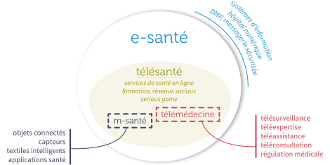
\includegraphics{img/circle.jpg}
\newline\newline
E sante : notion beaucoup plus large que la telesante
\newline
Telemedecine : necessite la presence d'un personnel medicale.
\newline\newline
Loi HPST(2009): telemedecine est une forme de pratique medicale a distance utilisant les technologies de l'information et de la communication. Elle met en rapport, entre eux ou avec un patient, un ou plusieurs professionels de sante, parmi les quels figure necessairement un professionel medical et le cas echeant, d'autres professionels apportait leurs soins aux patients.
\end{document}
